\section{Implementation}
\label{sect:kegg_implementation}

The implementations for \mawapp and \keggapp similar in many ways, but they have
some important differences. Development on \keggapp was begun a year after
\mawapp and provided opportunities to improve on the interface, design, and
implementation of the pathway viewing app concept.

The improved design was made possible partially by new features introduced into
the iPad development environmeng in 2011 with the release of iOS 5. The most
important change was ``automatic reference counting,'' (ARC) which moves memory
management responsibility from the programmer to the compiler. (See section
\ref{sect:objc_memory} for more information on ARC).

\keggappp architecture consists of a few well-defined components:

\begin{itemize}

    \item Top-level user interface such as the master-detail view
    
    \item Web service request classes that make HTTP requests to the PathCase
        KEGG server, process the response, and notify other objects of the
        results

    \item Views of specific kinds of data such as pathways (the main graph
        view), pathway lists, organism hierarchies, web pages, and pathway nodes

    \item Encapsulated components for specific functionality such as reading the
        ENZYME database and generating dynamic layouts with Graphviz

\end{itemize}

\subsection{Top-Level User Interface}
\label{sect:kegg_impl_top_level_ui}

\emph{To be written. This will be very similar in style to section
\ref{sect:maw_interface}.}

\subsection{Web Services}
\label{sect:kegg_impl_web_services}

There are four differences between the strategies of \mawapp and \keggapp
with respect to how web services are integrated into the application
architecture.

The first difference is that \keggapp does not download the entire PathCase
KEGG database at once. HTTP requests are made as new data is needed, and the
result is cached in the device's internal storage.

The second is in class hierarchy. \mawapp has methods in various data model
classes which are responsible for making an HTTP request and taking some action
based on its success or failure. \keggapp has a separate class for each web
service, named \texttt{PC<WebService>Fetcher}.

The third is how dependencies between requests are managed. \mawapp uses
mutexes to force the data update thread to wait before starting a request that
depends on a previous request. \keggappp web service classes fire events to
a central notification system when they have completed, and controller objects
check to see if any new web services should be invoked due to dependencies being
made available.

The fourth is in what sorts of transformations are done to the results of the
HTTP request. Unlike \mawapp, after the XML response has been parsed into
one or more KEGG internal objects, these objects are not serialized. In other
words, all objects generated by web services are built from the XML each time
they are needed. The XML response of the web service is the canonical
representation of the object.

These differences are summarized in figure
\ref{fig:kegg_impl_web_service_differences}.

\begin{figure}[hbt]
    \center{
        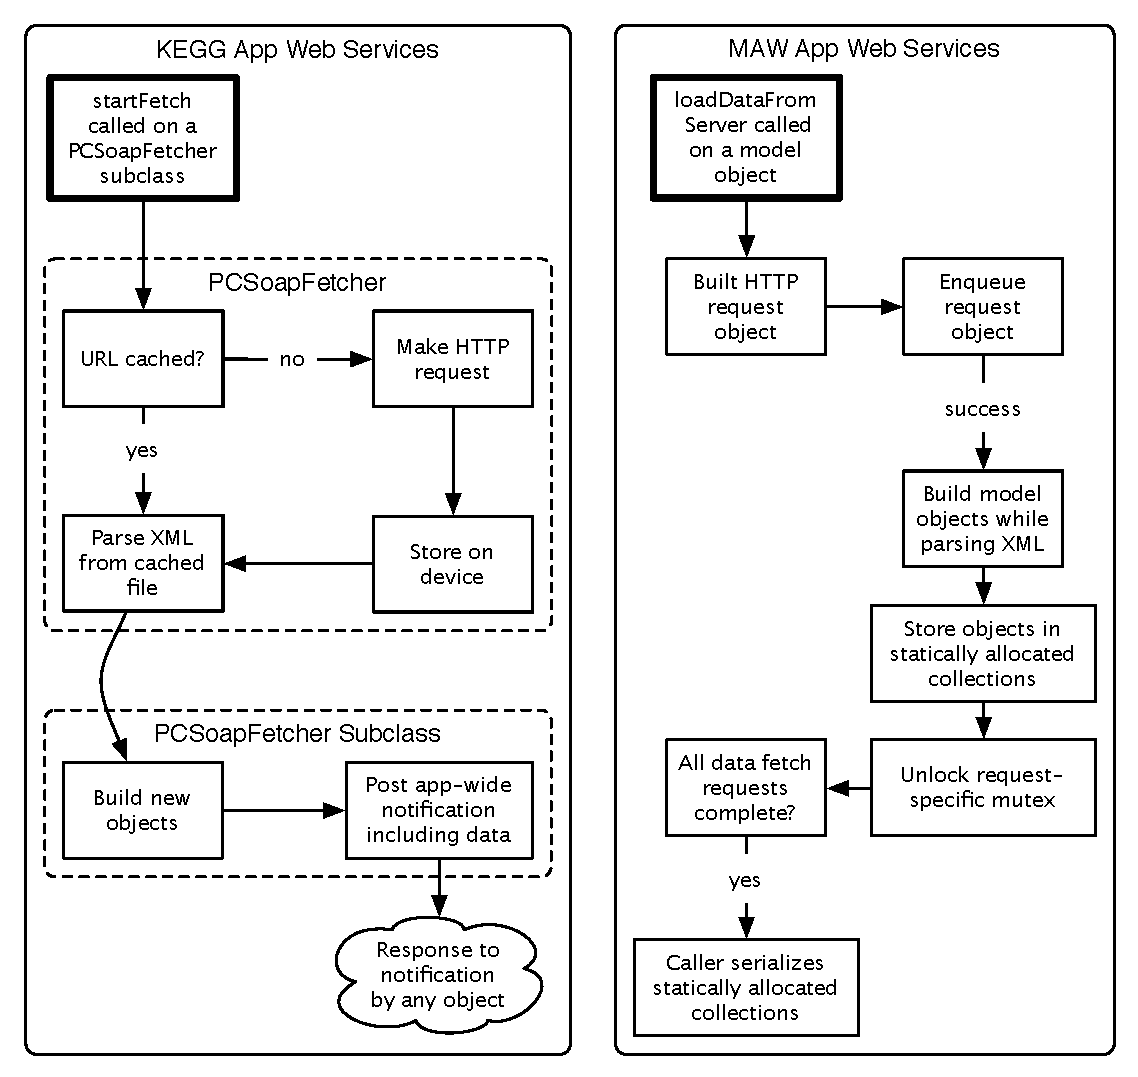
\includegraphics[width=\textwidth]{kegg/figures/web_services.pdf}}
    \caption{\label{fig:kegg_impl_web_service_differences} Side-by-side
    comparison of the typical life cycle of a \keggapp web service request and
    a \mawapp web service request.}
\end{figure}

This model of web services would not necessarily work better for \mawapp,
which needs quicker access to much more interdependent data. When the data model
is serialized, it is simple to load it and traverse complex relationships. The
data handled by \keggapp, on the other hand, is not very interdependent, so
it is simpler to make the web service requests on demand and turn the XML into
objects in memory on the fly.

\subsubsection{Pathway Graph View}
\label{sect:kegg_impl_graph_view}

\emph{This will be an explanation of the \keggapp graph view and how it differs
from the \mawapp graph view. It will explain the node and edge objects that are
used to construct and render the graph view, which are referred to later in this
chapter.}

\subsection{Reading the ENZYME Database}
\label{sect:kegg_impl_enzyme}

The ENZYME database is provided in a flat text file format
\cite{enzyme:enzuser}.  This format is not acceptable for random seeking
behavior, so it has been converted to a SQLite database \cite{sqlite:main} for
more efficient access.  SQLite is a minimal implementation of SQL intended to be
used as a storage medium for single-instance applications \cite{sqlite:main}.

Each line in the ENZYME database begins with a two-letter code identifying the
type of data on the line \cite{enzyme:enzuser}. The rest of the line contains
the data. These are the different line codes according to the user manual:

\begin{objc}
ID  Identification                         (Begins each entry;
                                            1 per entry)
DE  Description (official name)            (>=1 per entry)
AN  Alternate name(s)                      (>=0 per entry)
CA  Catalytic activity                     (>=1 per entry)
CF  Cofactor(s)                            (>=0 per entry)
CC  Comments                               (>=0 per entry)
PR  Cross-references to PROSITE            (>=0 per entry)
DR  Cross-references to Swiss-Prot         (>=0 per entry)
//  Termination line                       (Ends each entry;
                                            1 per entry)
\end{objc}

\keggapp uses the description, alternate name, catalytic activity, cofactor, and
comments, ignoring the remaining fields.

The user manual uses this example to demonstrate the file format:

\begin{objc}
ID   1.14.17.3
DE   Peptidylglycine monooxygenase.
AN   PAM.
AN   Peptidyl alpha-amidating enzyme.
AN   Peptidylglycine 2-hydroxylase.
AN   Peptidylglycine alpha-amidating monooxygenase.
CA   Peptidylglycine + ascorbate + O(2) = peptidyl(2-hydroxyglycine) +
CA   dehydroascorbate + H(2)O.
CF   Copper.
CC   -!- Peptidylglycines with a neutral amino acid residue in the penultimate
CC       position are the best substrates for the enzyme.
CC   -!- The product is unstable and dismutates to glyoxylate and the
CC       corresponding desglycine peptide amide, a reaction catalyzed by
CC       EC 4.3.2.5.
CC   -!- Involved in the final step of biosynthesis of alpha-melanotropin and
CC       related biologically active peptides.
PR   PROSITE; PDOC00080;
DR   P08478, AMD1_XENLA ;  P12890, AMD2_XENLA ;  P83388, AMDL_CAEEL ;
DR   P10731, AMD_BOVIN  ;  P19021, AMD_HUMAN  ;  P97467, AMD_MOUSE  ;
DR   P14925, AMD_RAT    ;  Q95XM2, PHM_CAEEL  ;  O01404, PHM_DROME  ;
//
\end{objc}

A separate program was written to convert this file format into a SQLite
database. The program is called
\href{https://github.com/irskep/enzyme2sqlite}{enzyme2sqlite}
\footnote{\href{https://github.com/irskep/enzyme2sqlite}{https:/\slash
github.com\slash irskep\slash enzyme2sqlite}} and is implemented in the Python
programming language.

The program runs in two steps. The first step parses the text file format with a
simple state machine. The second step inserts the parsed data row by row
into a SQLite database. This database has fields that correspond directly to the
fields in the text file.

Access to the SQLite database in \keggapp is encapsulated in the
\texttt{EKEnzyme} class, which can open connections to the SQLite database and
query it for individual enzyme information. It can be used by calling
\texttt{[EKEnzyme enzymeForID:(NSString *)ECNumber]}, which returns an
\texttt{EKEnzyme} object with attributes for each field in its corresponding
ENZYME database entry.

For example, to get the list of alternate names for peptidylglycine
monooxygenase, one would call \texttt{[[EKEnzyme enzymeForID:@``1.14.17.3'']
altNames]}.

\subsection{Dynamic Layouts with Graphviz}
\label{sect:kegg_impl_graphviz}

PathCase KEGG contains human-curated frozen layouts for some pathways, but not
all. In order to display the pathways without frozen layouts, \keggapp
uses the Graphviz library.

Graphviz is a system which, among other things, provides graph layout and
visualization functions \cite{graphviz}. It provides both command line and
programmatic interfaces for entering, laying out, and rendering graphs.

\keggapp encapsulates the layout functionality of the Graphviz library in a
class called \texttt{GVGraph}. An instance of this class represents a graph with
nodes, a label for each node, and one-directional edges that connect nodes.

To generate a layout, a \texttt{GVGraph} object must be created, and nodes and
edges must be added to it. This is accomplished by calling its methods
\texttt{addNodeWithID:label:} and \texttt{addEdgeWithHeadID:tailID:}. These
methods create internal \texttt{GVGraphNode} and \texttt{GVGraphEdge} objects
that represent the nodes and edges. These objects have no information about
color, shape, or other style attributes because those attributes are not
relevant to generating a layout.

Nodes and edges are added by calling methods on this class, which create
\texttt{GVGraphNode} and \texttt{GVGraphEdge} objects that contain only the
information that is important for generating a layout. They are completely
separate from the graph view node and edge objects that have additional
information about color and edge arrow shapes.

The dynamic layout is performed by calling the \texttt{computeLayoutWithEngine:}
method on the \texttt{GVGraph} instance. The argument to this function is a
constant representing either a spring-based or hierarchical layout engine. This
method converts the \texttt{GVGraphNode} and \texttt{GVGraphEdge} objects into
Graphviz's internal graph representation, asks Graphviz to generate a layout,
and reads the results back into the \texttt{GVGraphNode} and
\texttt{GVGraphEdge} objects. The caller may then read back the position data
from the \texttt{GVGraph} instance to use however it pleases.

To clarify these steps, here is the actual implementation of the dynamic layout
function in \keggapp, which applies a dynamic layout to the graph model
described in section \ref{sect:kegg_impl_graph_view}.

\begin{objc}
- (void)computeDynamicLayout
{
    GVGraph *g = [[GVGraph alloc] init];
    
    for (PCGraphNode *node in [self.nodes objectEnumerator]) {
        [g addNodeWithID:node.identifier label:node.label];
    }
    
    for (PCGraphEdge *edge in [self.edges objectEnumerator]) {
        [g addEdgeWithHeadID:edge.target.identifier tailID:edge.source.identifier];
    }
    
    [g computeLayoutWithEngine:GVLayoutEngineNeato];
    
    for (PCGraphNode *node in [self.nodes objectEnumerator]) {
        CGPoint position = [g positionForNodeID:node.identifier];
        node.position = position;
    }
}
\end{objc}
